\section{Focusing the LMT}

\subsection{}
Like all telescopes, the LMT must be focused several times a night.
To do this we make a small map of a bright point-like source and then adjust the z-position of the secondary mirror until the point spread function (the telescope’s response function) is round and maximized. 
% In this problem you will focus the telescope using actual data taken on February 7, 2015.

We are given 5 maps of a bright source taken on February 7, 2015. Along with them, we are given other 5 fits files which are the corresponding weights, $(1/\sigma^2)$, of the bright source maps.

We can use the Levenberg-Marquardt (LM) method \footnote{lmfit python package} to fit the point source maps to a 2D Gaussian. The LM method is a way to minimize the $\chi^2$ function using a seamless transition from the steepest descent method (STM) and the inverse Hessian method (IHM).

The bright source maps can be fitted to a 2D Gaussian described by the following equation
\begin{equation}
    f(x,y)=Ae^{-a(x-x_0)^2-b(x-x_0)(y-y_0)-c(y-y_0)^2}
\end{equation}
where 
\begin{align}
    a=\frac{\cos^2\theta}{2\sigma_x^2}+\frac{\sin^2\theta}{2\sigma_y^2}\\
    b=-\frac{\sin 2\theta}{2\sigma_x^2}+\frac{\sin 2\theta}{2\sigma_y^2}\\
    c=\frac{\sin^2\theta}{2\sigma_x^2}+\frac{\cos^2\theta}{2\sigma_y^2},
\end{align}
$A$ is the amplitude, $(x_0,y_0)$ is the center of the peak and $\theta$ is a rotation angle.

We can use LM method by the lmfit python package to find the best parameters that minimizes the $\chi^2$ function. 
These best values are then use to determine the Gaussian model for each map.
Figure \ref{fig:lmtRaw} shows the raw maps, the fitted map using the best values of the parameters $A,x_0,y_0,\sigma_x,\sigma_y,$ and $\theta$ and a map of the residuals. 

After this we plot the amplitude obtained from the best fit and its corresponding z-position of the secondary mirror. 

% The data is stored in the file maps.tar.gz on the class Moodle page. You can unpack that on a linux computer with the commands: gunzip maps.tar.gz and tar -xcv maps.tar. This will give you a set of 10 fits files (remember fits from homework 1) that you will read. The files with “signal” in the name are the maps of the source. The files with "weight" in the name are images with each pixel representing the weight $(1/\sigma^2)$ of each pixel in the corresponding signal map.

Putting all this together, use the lmfit Levenberg-Marquardt fitting package to fit each image to a 2-d gaussian. 
Find the best fit amplitude in each case and fit the best fit amplitudes to the function
\begin{equation}
    f(z)=a_0+a_1z+a_2z^2
\end{equation}
where z is the z-position of the secondary as given in the table below.

Use the results of this
fit to determine the best-fit position of the LMT's secondary mirror.

\begin{table}[h]
    \centering
    \begin{tabular}{|c|c|}
        \toprule
         Observation  & z-position (mm)  \\
         \midrule
         35114 & -3.0\\
         35115 & -2.0 \\
         35116 & -1.0 \\
         35117 & 0.0 \\
         35118 & 1.0\\
         \bottomrule
    \end{tabular}
    %\caption{Caption}
    %\label{tab:my_label}
\end{table}

\begin{figure}
    \centering
    \begin{subfigure}[b]{.5\textwidth}
        \centering
        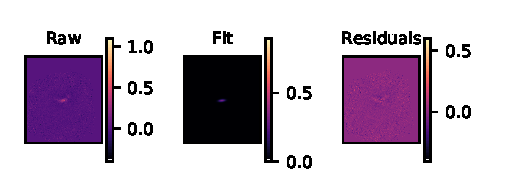
\includegraphics[height=100pt]{CodeAndFigures/DataFits4.pdf}
        \caption{Data:35114}
        \label{fig:lmtFit4}
    \end{subfigure}
    \begin{subfigure}[b]{.5\textwidth}
        \centering
        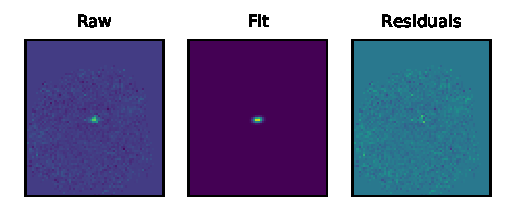
\includegraphics[height=100pt]{CodeAndFigures/DataFits5.pdf}
        \caption{Data:35115}
        \label{fig:lmtFit5}
    \end{subfigure}
    \begin{subfigure}[b]{.5\textwidth}
        \centering
        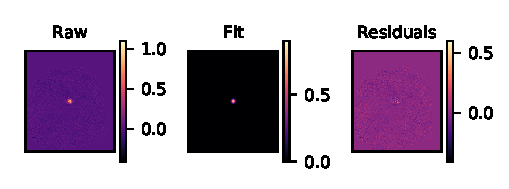
\includegraphics[height=100pt]{CodeAndFigures/DataFits6.pdf}
        \caption{Data:35116}
        \label{fig:lmtFit6}
    \end{subfigure}
    \begin{subfigure}[b]{.5\textwidth}
        \centering
        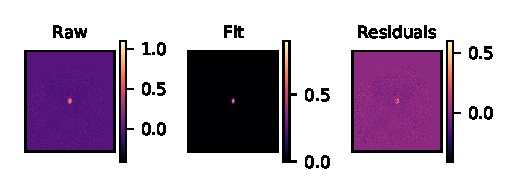
\includegraphics[height=100pt]{CodeAndFigures/DataFits7.pdf}
        \caption{Data:35117}
        \label{fig:lmtFit7}
    \end{subfigure}
    \begin{subfigure}[b]{.5\textwidth}
        \centering
        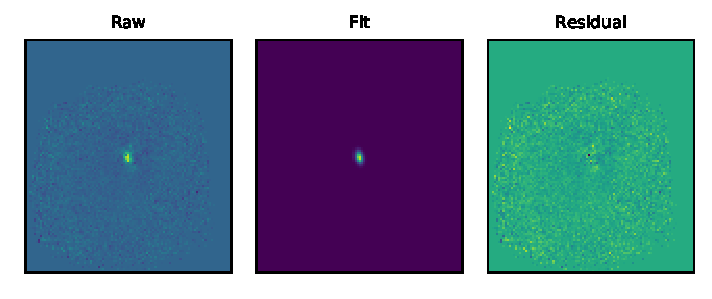
\includegraphics[height=100pt]{CodeAndFigures/DataFits8.pdf}
        \caption{Data:35118}
        \label{fig:lmtFit8}
    \end{subfigure}
    \caption{Image of the raw data, its 2D Gaussian fit and its residuals.}
    \label{fig:lmtRaw}
\end{figure}


\begin{figure}
    \centering
    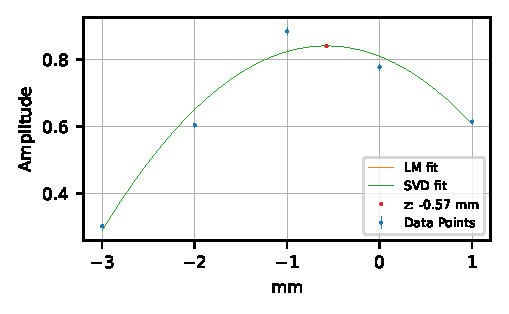
\includegraphics{CodeAndFigures/QuadFitPlot.pdf}
    \caption{Caption}
    \label{fig:lmtquadfit}
\end{figure}

\subsection{}

Use either the procedure outlined in the class18 notes or the emcee
python package to simulate the posterior probability distributions for all of the fitted parameters
in one of the 2-d gaussian fits you did. Describe what you see.